\subsubsection{Постановка задачі}
\begin{figure}[ht!]
    \begin{center}
        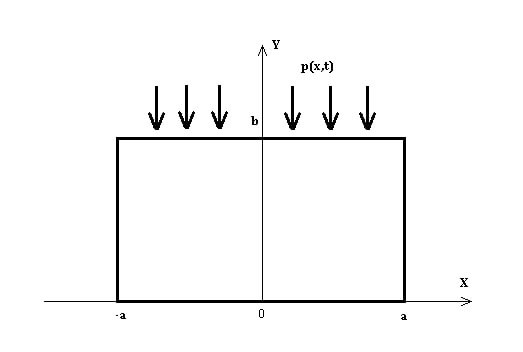
\includegraphics[scale=1]{images/geometry/image_1.jpg}
    \end{center}
    \caption{Геометрія проблеми}\label{geom_static_2}
\end{figure}
Розглядається пружне прямокутне тіло (Рис: \ref{geom_static_2}), яке займає облась,
що описується у декартовій системі координат співвідношеннями $-a \le x \le a$, $0 \le y \le b$.

На грані $y=b$ додане нормальне навантаження
\begin{equation}\label{bound_1_static_2}
    \sigma_y(x, y) |_{y=b} = -p(x), \quad  \tau_{xy}(x,y) |_{y=b} =0
\end{equation}
де $p(x)$ відома функція.

На бічних гранях виконуються умови другої основної задачі теорії пружності
\begin{equation}\label{bound_2_static_2}
    u(x,y) |_{x=\pm a} = 0, \quad v(x,y) |_{x=\pm a} =0
\end{equation}
На нижній грані виконується умова ідеального контакту
\begin{equation}\label{bound_3_static_2}
    v(x,y) |_{y=0} = 0, \quad \tau_{xy}(x,y) |_{y=0} =0
\end{equation}
Потрібно відшукати розв'язок рівняннь рівноваги
\begin{equation}\label{lame_static_2}
    \begin{cases}
        \frac{\partial^2 u(x,y)}{\partial x^2} + \frac{\partial^2 u(x,y)}{\partial y^2} + \mu_0 (\frac{\partial^2 u(x,y)}{\partial x^2} + \frac{\partial^2 v(x,y)}{\partial x\partial y}) = 0 \\
        \frac{\partial^2 v(x,y)}{\partial x^2} + \frac{\partial^2 v(x,y)}{\partial y^2} + \mu_0 (\frac{\partial^2 u(x,y)}{\partial x \partial y} + \frac{\partial^2 v(x,y)}{\partial y^2}) = 0 \\
    \end{cases}
\end{equation}
за умови виконання \eqref{bound_1_static_2} - \eqref{bound_3_static_2}

Щоб розв'язати поставлену задачу буде розглянуто половона прямокутної області $0 \le x \le a$, $0 \le y \le b$
та використовуючи властивості симметрії граничні умови на бічних гранях будуть мати наступний вигляд
\begin{equation}\label{bound_4_static_2}
    u(x,y) |_{x=0} = 0, \quad \tau_{xy}(x,y) |_{x=0} =0
\end{equation}
\begin{equation}\label{bound_5_static_2}
    u(x,y) |_{x=a} = 0, \quad v(x,y) |_{x=a} = 0
\end{equation}

\subsubsection{Розв'язання векторної крайовою задачі у просторі трансформант}
Для того, щоби звести задачу до одновимірної задачі, використано інтегральне перетворення Фур'є за змінною $x$ до рівнянь (\ref{lame_static_2}) наступному вигляді:
\begin{equation}
    \begin{pmatrix}
        u_n(y) \\
        v_n(y)
    \end{pmatrix} = \int_{0}^{a} 
    \begin{pmatrix}
        u(x,y) sin(\alpha_n x) \\
        v(x,y) cos(\alpha_n x)
    \end{pmatrix} dx, \quad \alpha_n = \frac{\pi n}{a}
\end{equation}

Для цього перше та друге рівняння (\ref{lame_static_2}) помножено відповідно на $sin(\alpha_n x)$ та $cos(\alpha_n x)$ та проінтегровано за змінною $x$ на інтервалі $0 \le x \le a$.

В результаті отримаємо наступну систему у просторі трансформант
\begin{equation}\label{transf_static_2}
    \begin{cases}
        u_n^{''}(y) - \alpha_n \mu_0 v_n^{'}(y) - \alpha_n^2 (1 + \mu_0) u_n(y) = 0 \\
        (1 + \mu_0) v_n^{''}(y) + \alpha_n \mu_0 u_n^{'}(y)  - \alpha_n^2 v_n(y) = -cos(\alpha_n) f(y) \\
    \end{cases},
\end{equation}
де $f(y) = \frac{\partial v(x,y)}{\partial x}|_{x=a}$ - невідома функція.

Крайові умови у просторі трансформант набувають вигляду
\begin{equation}\label{transf_bound_static_2}
    \begin{cases}
        \left( (2G + \lambda)v_n^{'}(y) + \alpha_n \lambda u_n(y) \right)|_{y=b} = -p_n, \\
        \left(u_n^{'}(y) - \alpha_n v_n(y)  \right)|_{y=b} = 0, \\
        v_n(y)|_{y=0} = 0, \\
        \left(u_n^{'}(y) - \alpha_n v_n(y)  \right)|_{y=0} = 0,
    \end{cases}
\end{equation}
де $p_n = \int_{0}^{a} p(x) cos(\alpha_n x) dx$.

Для того щоб розв'язати задачу у простосторі трансформант, перепишемо її у векторній формі.
Рівняння рівноваги (\ref{transf_static_2}) запишемо у наступному вигляді:
\begin{equation}\label{transf_mat_static_2}
    L_2\left[ Z_n(y) \right] = F_n(y)
\end{equation}
\begin{equation}
    L_2\left[ Z_n(y) \right] = A * Z_n^{''}(y) + B * Z_n^{'}(y) + C * Z_n(y) \nonumber \\
\end{equation}
де
\begin{equation*}
    A = \begin{pmatrix}
        1 & 0 \\
        0 & 1 + \mu_0
    \end{pmatrix}, \quad
    B = \begin{pmatrix}
        0 & -\alpha_n \mu_0 \\
        \alpha_n \mu_0 & 0
    \end{pmatrix}, \quad
    C = \begin{pmatrix}
        -\alpha_n^2(1 + \mu_0) & 0 \\
        0 & -\alpha_n^2
    \end{pmatrix}
\end{equation*}
\begin{equation*}
    Z_n(y) = \begin{pmatrix}
        u_n(y) \\
        v_n(y)
    \end{pmatrix}, \quad 
    F_n(y) = \begin{pmatrix}
        0 \\
        - cos(\alpha_n a) f(y)
    \end{pmatrix}
\end{equation*}
Граничні умови (\ref{transf_bound_static_2}) запишемо у наступному вигляді:
\begin{equation}\label{transf_bound_mat_static_2}
    U_i\left[ Z_n(y) \right] = D_i
\end{equation}
\begin{equation}
    U_i\left[ Z_n(y) \right] = E_i * Z_n^{'}(b_i) + F_i * Z_n(b_i) \nonumber \\
\end{equation}
де $i = \overline{0, 1}$, $b_0 = b$, $b_1 = 0$,
\begin{equation*}
    E_0 = \begin{pmatrix}
        1 & 0 \\
        0 & 2G + \lambda
    \end{pmatrix}, \quad
    F_0 = \begin{pmatrix}
        0 & -\alpha_n \\
        \alpha_n \lambda & 0
    \end{pmatrix}, \quad
\end{equation*}
\begin{equation*}
    E_1 = \begin{pmatrix}
        1 & 0 \\
        0 & 0
    \end{pmatrix}, \quad
    F_1 = \begin{pmatrix}
        0 & -\alpha_n \\
        0 & 1
    \end{pmatrix}, \quad
\end{equation*}
\begin{equation*}
    D_0 = \begin{pmatrix}
        0 \\
        -p_n
    \end{pmatrix}, \quad
    D_1 = \begin{pmatrix}
        0 \\
        0
    \end{pmatrix}, \quad
\end{equation*}

Розв'язок векторної одновимірної крайової задачі знайдено як суперпозиція загального розв'язку векторного однорідного рівняння $Z_n^0(y)$
та часткового розв'язку неоднорідного рівняння $Z_n^1(y)$.
\begin{equation}
    Z_n(y) = Z_n^0(y) + Z_n^1(y)
\end{equation}

Ці розв'язки знайдено за допомогою апарату матричного диференціального числення \cite{popov_4}, \cite{gantmaher},
для чого побудовано фундаментальну матричну систему розв'язків та фундаментальну базисну систему розв'язків відповідної матричної крайової задачі.

Потрібно відшукати розв'язок однорідного векторного рівняння \eqref{transf_mat_static_2}.
З цією метою спочатку розшукуємо розв'язок однорідного матричного рівняння.
Його побудовано у вигляді \cite{gantmaher}:
\begin{equation}
    Y(y) = \frac{1}{2\pi i} \oint_C e^{sy} M^{-1}(s)ds
\end{equation}
Де $M(s)$ - характерестична матриця рівняння (\ref{transf_mat_static_2}), $C$ - замкнений контур який містить усі особливі точки підінтегрального виразу.
Матрицю $M(s)$ знайдено з наступної умови
\begin{equation}
    L_2\left[ e^{sy}*I \right] = e^{sy} * M(s), \quad I = \begin{pmatrix} 1 & 0 \\ 0 & 1 \end{pmatrix},
\end{equation}
де матриця $M(s)$ має вигляд
\begin{equation}
    M(s) = \begin{pmatrix}
        s^2 -\alpha_n^2(1 + \mu_0) & -\alpha_n \mu_0 s \\
        \alpha_n \mu_0 s & s^2 (1 + \mu_0) -\alpha_n^2
     \end{pmatrix}
\end{equation}
Обернену матрицю $M^{-1}(s)$ знайдено у наступному поданні $M^{-1}(s) = \frac{\widetilde{M(s)}}{det[M(s)]}$, 
де $\widetilde{M(s)}$ - транспонована матриця алгебричних доповнень
\begin{equation}
    \widetilde{M(s)} = \begin{pmatrix}
        s^2 (1 + \mu_0) -\alpha_n^2 & \alpha_n \mu_0 s \\
        -\alpha_n \mu_0 s & s^2 -\alpha_n^2(1 + \mu_0)
     \end{pmatrix}
\end{equation}
$det[M(s)]$ - детермінант матриці
\begin{align}
    &det[M(s)] = \begin{vmatrix}
        s^2 - \alpha_n^2 - \alpha_n^2\mu_0 & -\alpha_n \mu_0 s \\
        \alpha_n \mu_0 s & s^2 (1 + \mu_0) -\alpha_n^2
     \end{vmatrix} = \nonumber \\
    &=(1+\mu_0)(s - \alpha_n)^2(s + \alpha_n)^2
\end{align}
де $-\alpha_n$, $\alpha_n$, корені другої кратності рівняння $det[M(s)]=0$, детальне знаходження яких наведено в (\nameref{ap_B}).

За допомогою теореми про лишки знайдено фундаментальну матричну систему
\begin{align*}
    &\frac{1}{2\pi i} \oint_C e^{sy} M^{-1}(s)ds = \frac{2 \pi i}{2 \pi i (1 + \mu_0)} \sum_{i=1}^{2} Res\left[ e^{sy} \frac{\widetilde{M(s)}}{det[M(s)]} \right] = \\
    & = \frac{1}{(1 + \mu_0)} \left(Y_0(y) + Y_1(y) \right)
\end{align*}
де
\begin{align}
    &Y_0(y) =  \frac{\partial}{\partial s} \left( \frac{e^{sy}}{(s+\alpha_n)^2} \widetilde{M(s)} \right) \Big|_{s=\alpha_n} = \nonumber \\
    &=\frac{e^{\alpha_n y}}{4\alpha_n} \begin{pmatrix}
    \alpha_n \mu_0 y + 2 + \mu_0 & \alpha_n \mu_0 y \\
    -\alpha_n \mu_0 y & -\alpha_n \mu_0 y + 2 + \mu_0
    \end{pmatrix}
\end{align}
\begin{align}
    &Y_1(y) = \frac{\partial}{\partial s} \left(\frac{e^{sy}}{(s-\alpha_n)^2} \widetilde{M(s)} \right) \Big|_{s=-\alpha_n} = \nonumber \\
    =&\frac{e^{-\alpha_n y}}{4\alpha_n} \begin{pmatrix}
    \alpha_n \mu_0 y - 2 - \mu_0 & -\alpha_n \mu_0 y \\
    \alpha_n \mu_0 y & -\alpha_n \mu_0 y - 2 - \mu_0
    \end{pmatrix}
\end{align}

Для побудови матриці-функції Гріна спочатку знайдено фундаментальну базисну систему розв'язків $\Psi_0(y)$, $\Psi_1(y)$, які мають задовільняти матричну крайову задачу \cite{popov_2}:
\begin{align}\label{psi_probl_static_2}
    &L_2\left[ \Psi_i(y) \right] = 0, \nonumber \\
    &U_i\left[ \Psi_j(y) \right] = \delta_{j,i}, \quad j= \overline{0, 1}, i= \overline{0, 1}
\end{align}

Для цього їх вибрано у формі:
\begin{equation}\label{psi_static_2}
    \Psi_i(y) = Y_0(y) * C_1^i + Y_2(y) * C_2^i,
\end{equation}
де $C_1^j$, $C_2^j$, $j=\overline{0, 1}$ невідомі матриці коєфіцієнтів, які знайдено з граничних умов \eqref{psi_probl_static_2}
(покрокове знаходження наведено у Додатку С).

Таким чином матрицю Гріна можемо записати у подані:
\begin{equation}\label{grin_matrix_static_2}
    G(y,\xi) = 
    \begin{cases}
        \Psi_0(y) * \Psi_1(\xi), \quad 0 \le y < \xi \\
        \Psi_1(y) * \Psi_0(\xi), \quad \xi < y \le b
    \end{cases}
\end{equation}

Для данної матриці Гріна виконано усі властивості, зокрема виконані однорідні граничні умови \eqref{transf_bound_mat_static_2}
та однорідні рівняння рівноваги у просторі трансформант \eqref{transf_mat_static_2}:
\begin{equation*}
    L_2\left[  G(y, \xi) \right] = 0
\end{equation*}
\begin{equation*}
    U_0\left[ G(y, \xi) \right] = 0, \quad  U_1\left[ G(y, \xi) \right] = 0,
\end{equation*}

Таким чином розв'язок неоднорідної векторної крайової задачі у просторі трансформант записано у поданні \cite{popov_2}
\begin{equation}
    Z_n(y) = \int_0^b G(y,\xi) F_n(\xi) d\xi + \Psi_0(y) * D_0 + \Psi_1(y) * D_1
\end{equation}

Введемо наступні позначення для матриці Гріна $G(y, \xi) = \begin{pmatrix}
    g_1(y,\xi) & g_2(y,\xi) \\
    g_3(y,\xi) & g_4(y,\xi)
\end{pmatrix}$,, $\Psi_i(y) = \begin{pmatrix}
    \psi_i^1(y) & \psi_i^2(y) \\
    \psi_i^3(y) & \psi_i^4(y)
\end{pmatrix}$, $i=0,1$.
Враховуючи це, шукані функціі перемішень у просторі трансформант представлено у наступному вигляді
\begin{align}\label{transf_sol_u_static_2}
    &u_n(y) = \int_0^b \left[g_1(y, \xi)f_n^1(\xi) + g_2(y, \xi)f_n^2(\xi) \right]d\xi - \psi_0^2(y) p_n
\end{align}
\begin{align}\label{transf_sol_v_static_2}
    &v_n(y) = \int_0^b \left[g_3(y, \xi)f_n^1(\xi) + g_4(y, \xi)f_n^2(\xi) \right]d\xi - \psi_0^4(y) p_n
\end{align}

Фінальний розв'язок вихідної задачі отримано після застосування оберненного перетворення Фур'є до трансформант \eqref{transf_sol_u_static_2}, \eqref{transf_sol_u_static_2}
\begin{equation}
    u(x,y) = \frac{2}{a} \sum_{n=1}^{\infty} u_n(y) sin(\alpha_n x), \quad \alpha_n = \frac{\pi n}{a}
\end{equation}
\begin{equation}
    v(x,y) = \frac{v_0(y)}{a} + \frac{2}{a} \sum_{n=1}^{\infty} v_n(y) cos(\alpha_n x), \quad \alpha_n = \frac{\pi n}{a}
\end{equation}

Знайдем тепер $v_0(y)$ розглянувши задачу у просторі трансформант \eqref{transf_static_2}, \eqref{transf_bound_static_2} при $n=0$, $\alpha_n = 0$.
Детальний розв'язок якої наведено в (\nameref{ap_D}). Тоді остаточний розв'язок $v(x,y)$ буде мати вигляд
\begin{align}
    &v(x,y) = \frac{2}{a} \sum_{n=1}^{\infty} v_n(y) cos(\alpha_n x) - \frac{p_0}{a(2G + \lambda)} - \\
    &- \frac{1}{a(1+\mu_0)} \int_{0}^{b}g(y,\xi) f(\xi) d\xi
\end{align}

\subsubsection{Розв'зання сингулярного інтегрального рівняння задачі}
Залишилось знайти невідому функцію $f(y)$ для якої побудовано сінгулярне інтегральне рівнняння за допомогою граничної умови $\sigma_y(x, y) |_{y=b} = -p(x)$.
\begin{equation}\label{int_eq_static_2}
    \frac{1}{\pi} \int_{-1}^{1} \left( a_2(t) ln\left[ \frac{1}{\lvert x - t \rvert} \right] + a_3(t, x) \right) f(t) dt = a_1(x),
\end{equation}
де
% нужно поправить
\begin{align*}
    &a_1(x) = a p(x) - 2(2G + \lambda) \frac{\partial}{\partial y} \sum_{n=1}^{\infty} \psi_0^{4}(y) p_n cos(\alpha_n x)|_{y=b} - \nonumber \\
    &- 2\lambda \frac{\partial}{\partial x} \sum_{n=1}^{\infty}\psi_0^2(y) p_n sin(\alpha_n x)|_{y=b} - \psi_0^{'}(b) p_0
\end{align*}
\begin{equation*}
    a_2(t) = \frac{2}{\pi} \lim_{n \rightarrow \infty}\left[ \frac{\partial \widetilde{g_4(y, \xi)}}{\partial y} + \lambda \widetilde{g_2(y, \xi)} \right]|_{y=b}, 
\end{equation*}
\begin{align*}
    &a_3(t, x) = \sum_{n=1}^{N} cos(\alpha_n a) cos(\alpha_n x) \left[(2G + \lambda) \frac{\partial g_4(y, t)}{\partial y} + \alpha_n \lambda g_2(y, t) \right]|_{y=b} - \\
    & - a_2 \sum_{n=0}^{N} (-1)^n (2n + 1)^{-1} e^{-(2n + 1) \frac{\pi}{2a} (b - t)} cos((2n + 1) \frac{\pi}{2a} x)
\end{align*}

Інтегральне рівняння \eqref{int_eq_static_2} розв'язується методом ортогональних поліномів \cite{popov_3}.
Згідно з методом невідому функцію $f(t)$ розвинуто у ряд за поліномами Чебишева першого роду
\begin{equation}\label{unk_fun_static_2}
    f(t) = \frac{1}{a_2(t)} \frac{1}{\sqrt{1 - t^2}} \sum_{k=0}^{\infty} \varphi_k T_{k}(t),
\end{equation}
де $\varphi_k$ - невідомі коєфіцієнти, $T_{k}(t)$ - поліном Чебишева першого роду.


Представлення невідомої функції \eqref{unk_fun_static_2} підставлено у сінгулярне інтегральне рівняння \eqref{int_eq_static_2}
та враховуючи спектральне співвідношення B.1.9 \cite{ortogonal}
\begin{equation}
    \frac{1}{\pi} \int_{-1}^{1} ln\left[ \frac{1}{\lvert x - t \rvert} \right] \frac{T_k(t)}{\sqrt{1 - t^2}} dt = \upsilon_k T_k(x),
    \begin{cases}
        \upsilon_0 = ln 2, \\
        \upsilon_k = k^{-1}, k \ge 1
    \end{cases}
\end{equation} 
отримано
\begin{equation}\label{int_eq_2_static_2}
    \sum_{k=0}^{\infty}  \varphi_k \upsilon_k T_{k}( x ) + \sum_{k=0}^{\infty} \varphi_k \frac{1}{\pi} \int_{0}^{1} \frac{a_3(t, x)}{a_2(t)} \frac{T_{k}(t)}{\sqrt{1 - t^2}} dt = a_1(x)
\end{equation}

Реалізація стандартної схеми методу ортогональних поліномів приводить до розв'язання нескінченої системи алгебричних рівнянь відносно невідномих коєфіцієнтів $\varphi_k$, $k=\overline{0, \infty}$,
яка в подальшому розв'язується методом редукції.

\begin{equation}\label{int_system_static_2}
    \frac{\phi_m \pi}{2m} + \sum_{k=0}^{\infty} \phi_k g_{k, m} = f_m,
\end{equation}
де $g_{k, m} = \frac{1}{\pi} \int_{-1}^{1} \frac{T_{m}(x)}{\sqrt{1 - x^2}} \int_{0}^{1} \frac{a_3(t, x )}{a_2(t)} \frac{T_{k}(t)}{\sqrt{1 - t^2}} dt dx$,
$f_m = \int_{-1}^{1} \frac{T_{m}(x) a_1(x)}{\sqrt{1 - x^2}} dx$ інтеграли відомих функцій

\subsubsection{Числові розрахунки та обговорення}
Наведені чисельні експеренти розглядаються для сталі ($E=200$ ГПА, $\mu=0.25$).

Розглянута прямокунта область $0 \le x \le 10$, $0 \le y \le 15$, при функції навантаження $p(x)=(x-2.5)^2$.
На малюнках (Рис: \ref{static_2_u_1}), (Рис: \ref{static_2_v_1}), (Рис: \ref{static_2_sigma_x_1}), (Рис: \ref{static_2_sigma_y_1})
представлені функіі переміщень $u(x,y)$, $v(x,y)$ та напружень $\sigma_x(x,y)$, $\sigma_y(x,y)$ відповідно.
\begin{figure}[h!]
    \begin{center}
        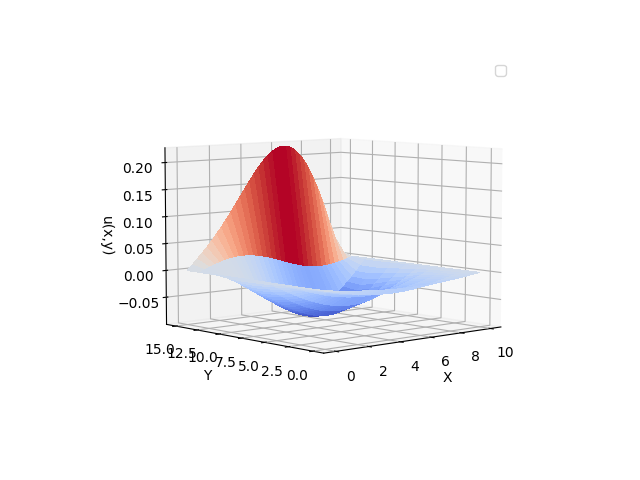
\includegraphics[width=0.49\textwidth, scale=1]{images/results/static_2/u_1.png}
        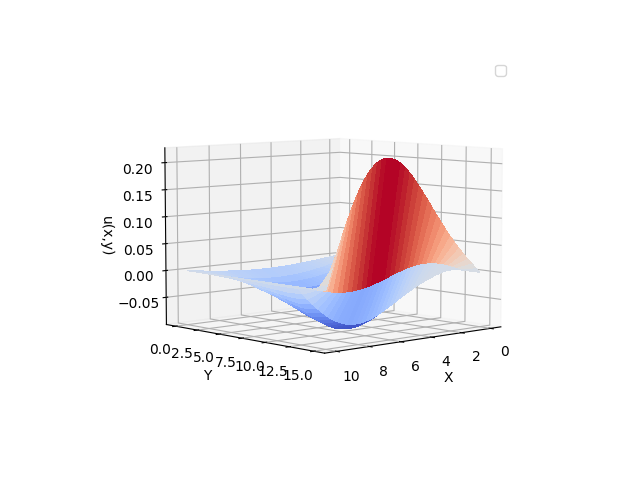
\includegraphics[width=0.49\textwidth, scale=1]{images/results/static_2/u_2.png}
        \caption{Функція $u(x, y)$}\label{static_2_u_1}
    \end{center}
\end{figure}
\newpage
\begin{figure}[h!]
    \begin{center}
        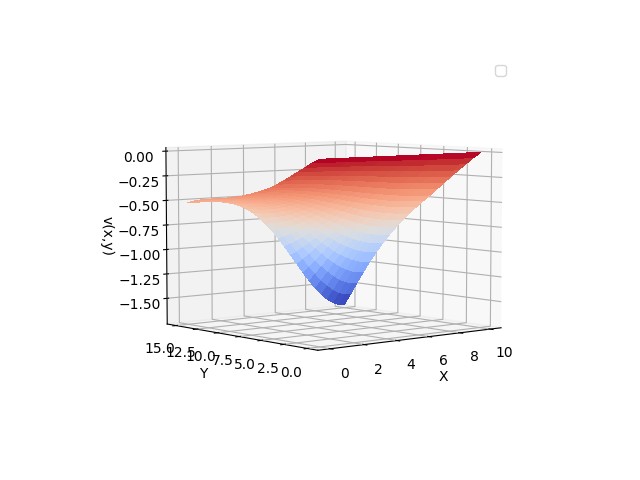
\includegraphics[width=0.49\textwidth, scale=1]{images/results/static_2/v_1.png}
        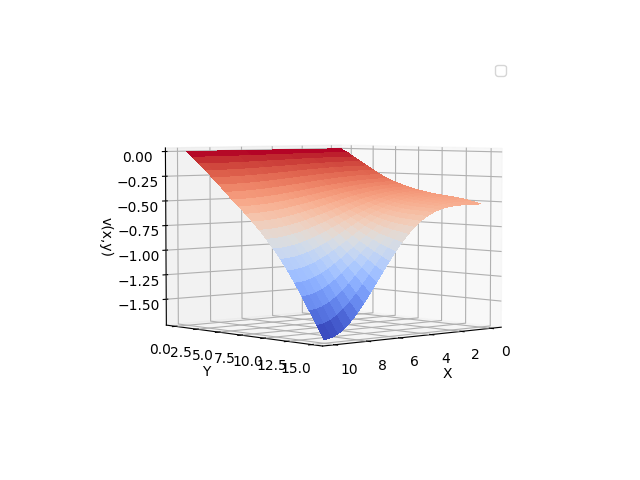
\includegraphics[width=0.49\textwidth, scale=1]{images/results/static_2/v_2.png}
        \caption{Функція $v(x, y)$}\label{static_2_v_1}
    \end{center}
\end{figure}
\begin{figure}[h!]
    \begin{center}
        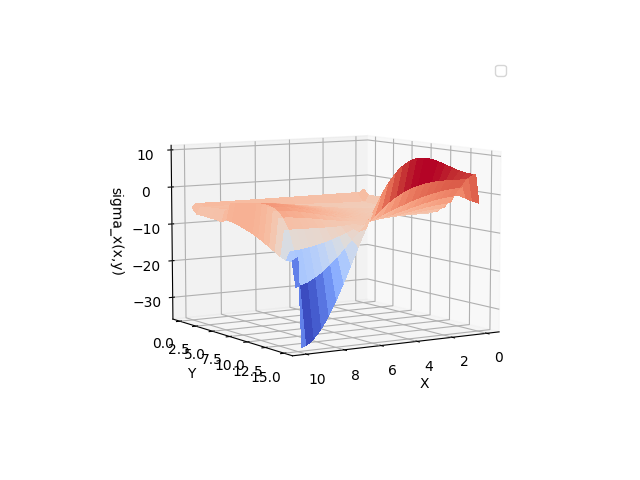
\includegraphics[width=0.49\textwidth, scale=1]{images/results/static_2/sigma_x_1.png}
        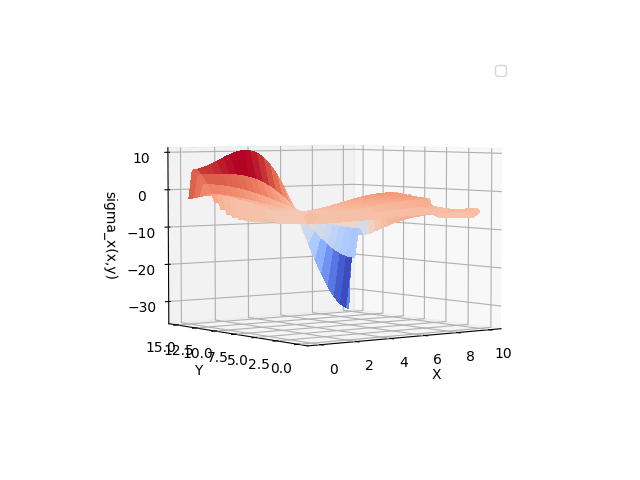
\includegraphics[width=0.49\textwidth, scale=1]{images/results/static_2/sigma_x_2.png}
        \caption{Функція $\sigma_x(x, y)$}\label{static_2_sigma_x_1}
    \end{center}
\end{figure}
\begin{figure}[h!]
    \begin{center}
        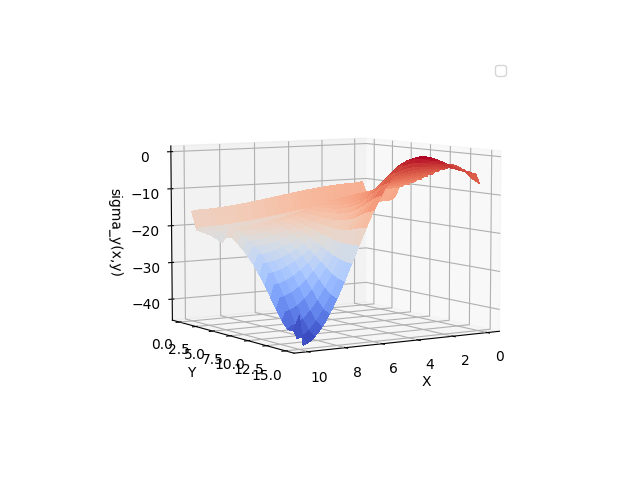
\includegraphics[width=0.49\textwidth, scale=1]{images/results/static_2/sigma_y_1.png}
        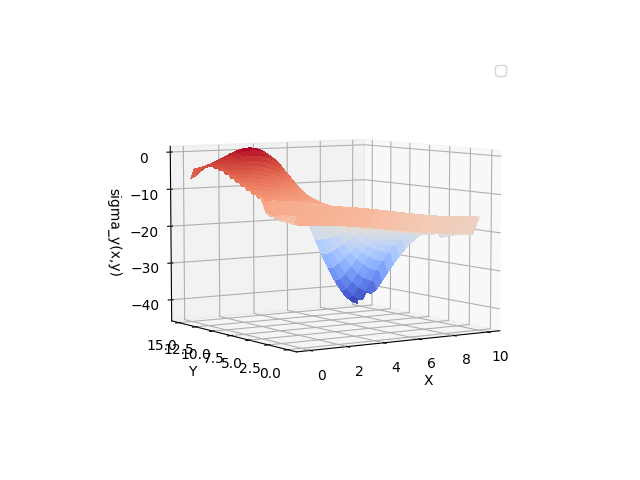
\includegraphics[width=0.49\textwidth, scale=1]{images/results/static_2/sigma_y_2.png}
        \caption{Функція $\sigma_y(x, y)$}\label{static_2_sigma_y_1}
    \end{center}
\end{figure}
